\documentclass[a4paper,10pt,spanish]{article}

% Preámbulo - Parte A

\usepackage[utf8]{inputenc} % Soporte para los acentos
\usepackage[T1]{fontenc}

\usepackage[spanish]{babel} % Capítulos, seciones, etc. en español

\usepackage[margin=2cm]{geometry} % Diseño del documento

\usepackage{multicol} % Escribir doble columna

\usepackage{xcolor} % Usar colores
\usepackage{pstricks}

\usepackage{enumerate} % Cambiar etiquetas de numeración
\usepackage[shortlabels]{enumitem} % Manejo adicional de etiquetas de numeración

\usepackage{graphicx} % Manejo de gráficos y figuras

\usepackage{makeidx} % Índice alfabético

% Paquetes adicionales de símbolos matemáticos
\usepackage{amsmath,amssymb,amsfonts,latexsym,cancel}

\usepackage{newcent}

\usepackage{listings}
\lstset{
basicstyle=\footnotesize\ttfamily
}

% Preámbulo - Parte B

\pagestyle{myheadings} % Numeración de página en la parte superior

\title{Sistemas Operativos} % Título
\author{Victor Franco Matzkin - Darién Julián Ramírez} % Autor
\date{\empty} % Fecha

% Cuerpo del documento

\begin{document}

\maketitle % Mostrar título

\tableofcontents

\clearpage

\section{Introducción a los Sistemas Operativos}

\subsection{Sistema Operativo}

Capa de software que se encarga de los recursos de la computadora para sus usuarios y aplicaciones. En sistemas de propósito general, los usuarios interactúan con las aplicaciones, las aplicaciones se ejecutan en un ambiente proporcionado por el SO y el SO controla el acceso al hardware. \\

¿Qué se necesita para que un SO pueda correr programas? \\

\subsection{Roles de un SO}

\begin{itemize} %Roles de un SO
\item \textit{Árbitro:} manejan recursos compartidos entre diferentes aplicaciones corriendo en la misma máquina (físicamente). Los SO aíslan las aplicaciones entre si de manera que un error en una no afecte a la otra, deben protegerse a si mismos y a las aplicaciones de virus, y al compartir recursos, deben decidir qué aplicaciones los obtienen.

\begin{quote}

\textbf{Compartir recursos:} (objetivos para SO)

	\begin{itemize}
	\item \textit{Alocar recursos:} el SO debe mantener las aplicaciones en simultáneo 	por separado, asignando recursos cuando sea necesario. Se debe proveer un 				multiplexado de recursos de manera de que la ejecución en un programa (que 				eventualmente requiera tiempo de procesamiento infinito) no impida el curso de las 	demás. Adicionalmente el usuario podría detener la ejecución de un programa que no 	responde.
	
	\item \textit{Aislamiento:} un error en una aplicación no puede interrumpir la 			ejecución de otros o del sistema operativo. Esto se denomina \textit{fault 				insolation} y requiere restringir el comportamiento de las aplicaciones de manera 		que no tengan control total del hardware.
	
	\item \textit{Comunicación:} proporcionar comunicación entre diferentes 				aplicaciones y usuarios. Se deben establecer límites que podrán ser cruzados de 		forma controlada por el SO.
	\end{itemize}

\end{quote}

\item \textit{Ilusionista:} los SO proporcionan una abstracción física para simplificar el diseño de las aplicaciones (por ejemplo, haciendo creer que la memoria es infinita, o que el microprocesador está dedicado enteramente). Esto permite que las aplicaciones sean creadas con un nivel de abstracción mayor y sea el SO el encargado de asignar o gestionar los recursos.

\begin{quote}

\textbf{Enmascarar limitaciones de hardware:} el hardware está limitado físicamente por lo que el SO debe decidir como dividir los recursos entre las diferentes aplicaciones en simultaneo. Un ejemplo es el uso del microprocesador, debiéndose proveer un método de virtualización (hacer creer a las aplicaciones que se dispone de recursos que no están presentes) y atomicidad (asegurar que las aplicaciones se realizan o no, y no quedar a medias).

\end{quote}

\item \textit{Glue:} conjunto de servicios entre aplicaciones para facilitar una apariencia o experiencia de usuario común (como copiar y pegar). Además los SO proporcionan una capa que separa las aplicaciones del hardware (para independizar aplicaciones de hardware en particular).

\begin{quote}

\textbf{Servicios en común:} el SO debe proporcionar servicios para facilitar el intercambio entre aplicaciones (por ejemplo, un servidor web debe ser capaz de leer un archivo escrito por el editor de texto) dependiendo de éste cuáles implementar (por ejemplo, las PC's pueden venir configuradas para funcionar con varios dispositivos diferentes -interfaces de red, discos, sensores, etc- y se usa una interfaz común pero en otras aplicaciones se podrá necesitar un nivel de abstracción menor).

Otro servicio estándar es la librería de la interfaz de usuario. Esto facilita a tener una apariencia similar en común, de manera que operaciones comunes (copiar y pegar) se manejen de forma consistente.

\end{quote}

\end{itemize} %Roles de un SO

\subsection{Patrones de diseño del SO}

Existen sistemas que si bien poseen otro dominio, deben cumplir tareas similares a los sistemas operativos (junto a las abstracciones):

\begin{itemize}
\item \textit{Cloud computing:} modelo a gran escala donde las aplicaciones se ejecutan en la nube (computadoras compartidas).

\item \textit{Navegadores:} muchas páginas web poseen \textit{scripts} (programas) que deben ser ejecutados por el navegador, por lo que éste debe aislar al usuario, a otros sitios y hasta al mismo navegador de actividad maliciosa (esto aumenta en el uso de extensiones).

\item \textit{Reproductores multimedia:} proveen un entorno de ejecución para programas en \textit{scripts}.

\item \textit{Sistemas de bases de datos multiusuario:} deben aislar los datos que no pueden ser vistos por determinados usuarios, que la información sea consistente, etc.

\item \textit{Aplicaciones paralelas:} éstas imponen un sistema en tiempo de ejecución sobre el SO para proporcionar paralelismo.

\item \textit{Internet.}
\end{itemize}

Todos estos sistemas deben proveer los tres roles de una forma en particular para funcionar.\\

\subsection{Desafíos de los SO}

\begin{itemize}
\item \textit{Confiabilidad:} el sistema hace lo que tiene que hacer, si hay errores el SO puede romperse o detenerse y perder la información, o gracias al aislamiento, la aplicación puede fallar ella sola y el SO manejar su reinicio. Este objetivo es difícil de lograr porque hay aplicaciones que se aprovechan de errores de implementación para tomar el control de sistema, por lo que se consigue mediante \textit{testing}.

\item \textit{Disponibilidad:} es el porcentaje de tiempo en el que el SO es usable. Está afectado por dos factores: frecuencia de fallas (MTTF), y el tiempo que tarda el sistema en reiniciarse luego de una falla (MTTR).

\item \textit{Seguridad:} es la propiedad de que el funcionamiento de la PC no pueda ser comprometido por un atacante malintencionado. Un SO debe minimizar su vulnerabilidad de ser atacado, pero también las aplicaciones deben seguir criterios de seguridad. El SO se asegura de que ciertas acciones estén permitidas a través del \textit{enforcement} (aplicación).

\item \textit{Privacidad:} es una parte de la seguridad, que establece que los datos almacenados sean accesibles por usuarios autorizados. Un política de seguridad define qué está permitido (quién puede acceder a cuáles datos y quién puede realizar cuáles operaciones).

\item \textit{Portabilidad:} una abstracción portable de un SO es una que no cambia cuando cambia el hardware (no volver a reinventar las aplicaciones o el SO), es decir, los SO's deben soportar aplicaciones que aún no han sido escritas para correr en hardaware todavía no desarrollado. Consiste en una forma simple y estándar de que las aplicaciones interactúen con el SO mediante una interfaz abstracta. La \textit{interfaz de máquina abstracta} (AMI) es la interfaz entre el sistema operativo y las aplicaciones. La \textit{interfaz de programación de aplicaciones} (API) es una parte de la AMI que es una lista de funciones que el SO da a las aplicaciones AMI, además incluye un modelo de acceso a la memoria y cuáles instrucciones pueden ser ejecutadas.\\
El concepto de portabilidad se extiende al mismo SO: éste puede ser implementado independientemente de los detalles de hardware. Esta interfaz se denomina \textit{capa de abstracción de hardware} (HAL).

\item \textit{Rendimiento:} el SO tiene un gran impacto en el rendimiento percibido de las aplicaciones porque éste decide qué y cuántos recursos va a utilizar. Una forma de medir el rendimiento es mediante la eficiencia (o inversamente el \textit{overhead} -el costo de recursos agregado por implementar una abstracción-), es ver el grado con el cual la abstracción impide el rendimiento de la aplicación.

\item \textit{Equidad (fairness):} es establecer una división equitativa de los recursos.

\item \textit{Tiempo de respuesta:} cuanto tarda una tarea desde que inicia hasta que se completa. Un concepto relacionado es el \textit{throughput}, que es la tasa en la cual un grupo de tareas se ejecuta.

\item \textit{Predictibilidad:} el tiempo de respuesta (u otra métrica) es consistente a través del tiempo.

\end{itemize}

\subsection{Sistemas Operativos MultiUsuarios}

Hay varias formas de compartir los recursos con muchos usuarios. Cuando se tiene un SO \textit{batch}, un programa se carga en memoria y en ese tiempo se ejecuta otro. Este SO se instala en la memoria y ejecuta un ciclo: \textit{cargar-ejecutar-descargar} para cada trabajo, y mientras se ejecuta uno, el SO puede comenzar a transferir mediante los dispositivos \textit{input-output} para el siguiente trabajo, a través del DMA (permite lear y escribir en la memoria independientemente del microprocesador).

Los sistemas \textit{batch} luego se extendieron para ejecutar varias aplicaciones al mismo tiempo (\textit{multitasking}). Se dice que el \textit{multitasking} mejora la eficiencia del microprocesador porque se tienen muchos programas en memoria al mismo tiempo, cada uno esperando a ser ejecutado. Para aumentar el aislamiento se agregó protección de memoria por hardware. \\

\subsection{Sistemas Operativos de tiempo compartido}

Son optimizados para los usuarios (y no el microprocesador) o mejor dicho, están diseñados para soportar el uso interactivo de la PC. El usuario usa los periféricos que envían interrupciones al microprocesador, interpreta los eventos y los manda a una cola del SO de manera que cuando la aplicación de usuario se ejecute, tome los eventos del SO, los procese, altere la salida visual y siga al evento siguiente. Los SO deben, por lo tanto, estar diseñados para ejecutar muchas actividades cortas. \\

\subsection{Sistemas Operativos Modernos}

\begin{itemize}
\item \textit{Escritorio:} poseen un usuario a la vez, varias aplicaciones, varios periféricos.

\item \textit{SO móviles:} un usuario, muchas aplicaciones, necesidad de aislamiento.

\item \textit{Sistemas embebidos:} los dispositivos embebidos ejecutan un SO a medida, con el software necesario para controlar el dispositivo.

\item \textit{Máquinas virtuales:} SO's que son ejecutados por otros SO's como si fueran una aplicación.

\item \textit{Servidores:} versiones industriales de los SO's de escritorio que operan en ambientes de red hostiles o donde hay mucho tráfico de red.

\item \textit{Clusters:} permiten descentralizar las tareas, ya que si un servidor falla, otro puede tomar el control, o también puede ejecutar partes de una misma tarea en simultaneo. Operan con una interfaz abstracta que aísla el software del hardware.
\end{itemize}

\section{Procesos}

\subsection{Protección}

Aislar las aplicaciones y el SO de las aplicaciones y usuarios potencialmente dañinos. Es esencial para lograr los objetivos de \textit{confiabilidad, seguridad, privacidad} y \textit{eficiencia}. Es implementada por el \textit{kernel} del sistema (nivel del software corriendo en el sistema, con acceso a todos los recursos de hardware). Todo lo que pueda no ser confiable deberá ejecutarse en un ambiente restringido con menores niveles de acceso (nivel de usuario). \\

\subsection{Proceso}

Es la abstracción de protección proporcionada por el \textit{kernel}, es decir, la ejecución de un programa con derechos restringidos. Este proceso necesita permiso del \textit{kernel} antes de acceder a la memoria de otro proceso, antes de leer o escribir en el disco, antes de cambiar la configuración de hardware, etc. \\

\subsection{Concepto de proceso}

En el caso general, un programador escribe código en un lenguaje de alto nivel. Luego un compilador convierte ese código en una secuencia de instrucciones de máquina, que se guardan en un archivo llamado \textit{imagen ejecutable}. Para iniciar el programa, el SO copia las instrucciones y datos de la imagen ejecutable a la memoria física. El SO separa también memoria para la pila de ejecución para almacenar el estado de las variables locales durante la llamada a procedimientos. También separa memoria para el \textit{heap} para cualquier estructura de datos u objetos dinámicos que el programa pueda necesitar. Al momento de cargar un programa a la memoria, el SO debe estar cargado en la misma con su pila y su \textit{heap}. Una vez que el programa está en la memoria, el SO lo puede ejecutar estableciendo el puntero de la pila y saltando a la primera instrucción del programa.

Si un usuario quiere ejecutar múltiples copias de un programa, el SO puede hacerlo copiando las instrucciones, datos estáticos, \textit{heap} y pila en memoria. Por lo tanto, \textit{la diferencia entre proceso y programa es que un proceso es una instancia de un programa con un estado}.

El SO sigue los procesos en ejecución usando una estructura de datos llamadas \textit{bloque de control de procesos}, que almacena toda la información que requiere de un proceso en particular (ubicación en memoria, en qué parte del disco se encuentra su imagen, usuario que lo ejecutó, privilegios, etc). \\

\subsection{Dual-Mode Operation}

Trabajar con dos modos permite que los programas puedan ser ejecutados y las instrucciones que son seguras de ejecutar corran directamente en el hardware, mientras que las demás se ejecuten en un modo restringido. Este modo se presenta mediante un bit en el registro de estado del microprocesador que indica el estado actual. En el \textit{modo usuario} el microprocesador se fija si la instrucción tiene permiso para ser ejecutada cuando es leída, mientras que en el \textit{modo kernel} no se realiza un control de seguridad.

Para que el \textit{kernel} pueda proteger las aplicaciones y usuarios mediante este mecanismo, el hardware debe soportar:

\begin{itemize}
\item \textit{Instrucciones privilegiadas:} instrucciones potencialmente peligrosas que no pueden ejecutarse en modo usuario.

\begin{quote}
El aislamiento de los procesos es posible si existe una forma de evitar que los programas en modo usuario cambien su nivel de privilegio. Las instrucciones con privilegios son aquellas que están sólo disponibles en \textit{modo kernel}. De esta forma el SO se ejecuta en \textit{modo kernel} mientras que las aplicaciones poseen un conjunto de instrucciones reducido. Si una aplicación intenta acceder a una posición de memoria que no le corresponde, o quiere cambiar su nivel de privilegio, ocurre una excepción en el microprocesador, que causa que el control quede en manos del \textit{exception handler} en el \textit{kernel}. Generalmente el SO interpreta esto como un bug y detiene la ejecución del programa.
\end{quote}

\item \textit{Protección de memoria:} en modo usuario, los accesos a memoria por afuera del proceso están prohibidos.

\begin{quote}
¿Cómo el SO previene que una aplicación acceda a partes de la memoria física (que no corresponden)?

Mediante mecanismos como \textit{base and bounds}. \textit{Base} es el inicio de la región de memoria del proceso y \textit{bounds} su longitud. Estos registros sólo pueden ser cambiados por instrucciones privilegiadas. Cada vez que el procesador toma una instrucción, se fija en la dirección del \textit{program counter} para ver si yace en los registros \textit{base and bounds}, si es así, la instrucción continúa, de lo contrario se lanza una excepción.

De todas formas, este sistema no permite las características:

\begin{itemize}
\item \textit{Heap} y pilas extensibles luego de cargar el programa en memoria.
\item Compartir memoria (al ejecutar varias instancias del mismo programa).
\item Direcciones de memoria absolutas (ya que todo es relativo a estas variables).
\item Fragmentación de memoria al no poder realocar los programas una vez iniciados.
\end{itemize}

El SO se ejecuta sin \textit{base and bounds}.

\end{quote}

\item \textit{Interrupciones por tiempo:} sin importar lo que haga el proceso, el \textit{kernel} debe tener una forma de tomar el control del proceso periódicamente.

\begin{quote}
\textit{Direcciones virtuales:}

Nivel de abstracción introducido por los microprocesadores en los que la memoria de los procesos comienzan en el mismo lugar y cada proceso cree que dispone de toda la memoria. El hardware se encarga de traducir las direcciones virtuales a físicas, de forma de solucionar los problemas anteriores. \\

\textit{Interrupciones por tiempo (timer interrupts)}: es una forma de que el sistema pueda terminar con la ejecución de un proceso, o ganar el control para cambiar a otra tarea. Se realiza mediante un \textit{hardware timer}, que interrumpe el microprocesador cada cierto tiempo o cantidad de instrucciones. Cuando ocurre una interrupción del \textit{timer} el control es transferido del proceso en \textit{modo usuario} al SO en \textit{modo kernel}. En la mayoría de los casos el SO resumirá la ejecución sin cambiar nada (modo, \textit{program counter}, registros).

Reiniciar el \textit{timer} es una instrucción privilegiada.
\end{quote}

\end{itemize}

\subsection{Transferir a \textit{modo seguro}}

Hasta aquí se tienen los procesos de usuario en un marco seguro, debiéndose establecer ahora cómo cambiar de modo, requiriendo un mecanismo seguro para no corromper el sistema. \\

\begin{minipage}[t]{0.45\linewidth}

\begin{center}
\fbox{De \textit{modo usuario} a \textit{modo kernel}}
\end{center} 

Hay \textit{tres} formas de que el \textit{kernel} tome el control desde un proceso:

\begin{itemize}
\item \textit{Excepciones:} condiciones inesperadas causadas por el comportamiento del programa. Cuando ocurren, el hardware detiene el proceso y deja el control en la \textit{exception handler}.

	\begin{itemize}
	\item Ejemplos: acceso a memoria no autorizados, división por cero, 						\textit{debugging} (break points).
	\end{itemize}
	
\item \textit{Interrupciones:} señales asíncronas que se envían al microprocesador indicando que ocurrió un evento externo y puede requerir su atención. Actúa de manera similar que en las excepciones, el microprocesador detiene el proceso en ejecución y comienza a ejecutarse en el \textit{kernel} mediante un \textit{interruption handler}. Cada tipo de interrupción tiene su \textit{handler}.

	\begin{itemize}
	\item Ejemplos: \textit{timer}, mouse/teclado, ethernet/wifi, discos.
	\end{itemize}

Una alternativa a las interrupciones es el \textit{polling}, que consiste en un ciclo de \textit{kernel} que verifica si ocurrió algún evento en los periféricos.

\item \textit{Llamadas al sistema:} son procedimientos del \textit{kernel} que pueden ser llamados a nivel de usuario (interrupciones \textit{trap}). Pueden ser ejecutados automáticamente luego de una excepción.

	\begin{itemize}
	\item Ejemplos: establecer conexión, intercambiar archivos en red, crear o 				modificar archivos, crear nuevos procesos.
	\end{itemize}

\end{itemize}

\end{minipage} \hfill \begin{minipage}[t]{0.45\linewidth}

\begin{center}
\fbox{De \textit{modo kernel} a \textit{modo usuario}}
\end{center}

En el caso inverso hay causas diferentes para efectuar la transición:

\begin{itemize}
\item \textit{Nuevo proceso:} luego de que el \textit{kernel} copia el programa en memoria, cambia el \textit{program counter} y el puntero de la pila, cambia a \textit{modo usuario}.

\item \textit{Continuar luego de una excepción, interrupción o llamada al sistema:} restaura el \textit{program counter} y sus registros, y cambia a \textit{modo usuario}.

\item \textit{Cambiar a otro proceso:} en algún caso el \textit{kernel} querrá cambiar el proceso actual por otro luego de una excepción, interrupción, etc. Para ello, el \textit{kernel} guarda el estado del proceso (\textit{program counter}, registros, etc) en el bloque de control de procesos. El \textit{kernel} carga estos datos del otro proceso y cambia a \textit{modo usuario}.

\item \textit{Upcall a nivel de usuario:} análogo a las interrupciones, pero al revés. Son mecanismos para que los programas de usuario reciban notificaciones o eventos asíncronos del \textit{kernel}.
\end{itemize}

\end{minipage} \\ \\

\subsection{Ejecutar procesos}

Para ejecutar aplicaciones a nivel de usuario el \textit{kernel} debe:

\begin{itemize}
\item Alocar e inicializar el bloque de control de proceso.
\item Alocar memoria para el proceso.
\item Copiar el programa del disco a la memoria recién alocada.
\item Alocar una pila para el nivel de usuario.
\item Alocar una pila para el nivel de \textit{kernel} para manejar \textit{llamadas al sistema}, \textit{interrupciones} y \textit{excepciones}.
\end{itemize}

Para ejecutar un programa, el \textit{kernel} también debe:

\begin{itemize}
\item Copiar argumentos a la memoria del usuario.
\item Transferir control al modo usuario.
\end{itemize}

\subsection{La interfaz de programación}

Falta definir cómo usar la abstracción del proceso, esto es, qué funcionalidades deben ponerse en el \textit{kernel}, cuáles debe brindar a las aplicaciones, qué debe ponerse en las bibliotecas de usuario, y cómo debe organizarse el SO. \textit{Esto es lo que distingue un SO de otro}. \\

\subsection{Funciones que debe proporcionar un SO}

\begin{enumerate}[a.]
\item \textit{Gestión de procesos:} ¿Un programa puede crear una instancia de otro? ¿Puede detener a otro programa? ¿Enviar un evento asíncrono?
\item \textit{Input/Output:} ¿Cómo se comunican los procesos con los periféricos? ¿Y entre procesos?
\item \textit{Manejo de hilos:} ¿Pueden crearse hilos que compartan memoria dado un proceso?
\item \textit{Manejo de memoria:} ¿Puede un proceso pedir memoria? ¿Puede compartirla con otros procesos?
\item \textit{Sistema de archivos y almacenamiento:} ¿Cómo un proceso guarda los datos de forma persistente?
\item \textit{Redes y sistemas distribuidos:} ¿Cómo un proceso controla pixeles? ¿Cómo se usan los aceleradores?
\item \textit{Autenticación y seguridad:} ¿Qué permisos tiene un programa y cómo se actualizan? ¿Cómo sabemos si el usuario es quién dice ser?
\end{enumerate}

\subsection{Implementación de las funciones del SO}

Las funciones antes descritas se pueden ubicar de diferentes formas:

\begin{enumerate}[a.]
\item Poner la funcionalidad en un programa en modo usuario.

	\begin{itemize}
	\item Ejemplo: programa para el login, para administrar procesos.
	\end{itemize}
	
\item En una librería a nivel de usuario que se enlaza con cada aplicación.

	\begin{itemize}
	\item Ejemplo: widgets de la interfaz de usuario (Win/Mac).
	\end{itemize}

\item En el \textit{kernel} que se accede con una llamada al sistema.

	\begin{itemize}
	\item Ejemplo: manejo de procesos, \textit{filesystem}/pila de red (Unix).
	\end{itemize}

\item Acceder a la función mediante una llamada al sistema e implementarla en un servidor invocado por el \textit{kernel}.

	\begin{itemize}
	\item Ejemplo: gestor de ventanas.
	\end{itemize}

\end{enumerate}

\subsection{Criterios para la implementación de las funciones}

\begin{enumerate}[I.]
\item \textit{Flexibilidad:} es más fácil cambiar el código del SO que se encuentra fuera del \textit{kernel}. Un cambio en la interfaz de las \textit{llamadas al sistema} implica cambios en el \textit{kernel} y las aplicaciones.

\item \textit{Seguridad:} la seguridad debe estar implementada en el \textit{kernel} (ya que si se hace en \textit{modo usuario} puede ser salteada).

\item \textit{Confiabilidad:} los módulos de \textit{kernel} no están protegidos entre sí, por lo que un error en el \textit{kernel} puede comprometer los datos de usuario y del \textit{kernel}, por lo que la confiabilidad se logra manteniendo un \textit{kernel} pequeño. En un diseño \textit{microkernel} las partes menos críticas del SO (sistema de archivos, ventanas) se aíslan del resto del \textit{kernel} resultando en un \textit{kernel} pequeño. Se pueden agregar nuevas características sin recompilar todo el \textit{kernel}. Por otro lado, los sistemas monolíticos son más rápidos pero son más grandes (deben almacenar los drivers en el espacio del \textit{kernel}), son más inseguros frente a los fallos de drivers (ya que pueden comprometer al sistema).

\item \textit{Rendimiento:} transferir en control al \textit{kernel} es más costoso que una llamada a una librería, por eso no prosperó el \textit{microkernel} de WinNT.
\end{enumerate}

\subsection{Administración de procesos}

En los primeros sistemas de procesamiento, el \textit{kernel} tenía el control por necesidad, siendo éste quien creaba los procesos a partir de las tareas que enviaba el usuario. Un enfoque diferente es permitir que los programas creen y administren sus propios procesos. \\

En Windows, se puede usar la función \texttt{createProcess()}, que en síntesis crea en inicializa el bloque de control de proceso en el \textit{kernel}, crea e inicializa un nuevo espacio de direcciones, carga el programa al espacio de direcciones, copia los argumentos en memoria al espacio de direcciones, inicializa el contexto de hardware para comenzar la ejecución y por último informa al planificador que el proceso está listo.

El proceso padre puede controlar los privilegios del hijo, donde enviar su \textit{Input/Output}, dónde almacenar los archivos, prioridad del planificador, etc. \\

En UNIX, se utiliza un enfoque diferente, dividiendo la tarea en dos pasos:

\begin{itemize}
\item \texttt{fork()}: crea una copia completa del proceso padre (se le da el control al ser una copia del padre), y el proceso hijo establece sus privilegios, prioridades y \textit{I/O} para el programa que se iniciará. Devuelve un entero.

\item \texttt{exec()}: carga la imagen ejecutable creada anteriormente y la ejecuta. Requiere como argumentos el nombre del ejecutable a correr y un arreglo de argumentos para pasarle al programa.
\end{itemize}

Para implementar \texttt{fork} en el \textit{kernel} hay que crear en inicializar el \textit{bloque de control de proceso} (PCB) en el \textit{kernel}, crear un espacio de direcciones, inicializar el espacio de direcciones con una copia de los contenidos del  espacio de direcciones del padre, heredar el contexto de ejecución del padre, e informar al planificador que hay un proceso listo para ejecutarse.

El \texttt{fork()} retorna valores dos veces: en el padre, devuelve el \textit{process ID} del hijo, y en el hijo retorna cero (éxito), de manera de saber quién es el hijo. Esta relación no establece que el hijo se ejecutará después del padre, ya que ambos procesos están listos y el padre puede quedar en espera por el \textit{timer}, por lo que el orden depende del planificador.

El \texttt{exec()} completa los pasos necesarios para correr el programa: cargar el programa al espacio de direcciones actual, copiar los argumentos a la memoria e inicializar el contexto de hardware para iniciar la ejecución.

Notar que no crea un nuevo proceso. En el caso de que el proceso padre requiera que el proceso hijo termine, se usa la \textit{llamada al sistema} \texttt{wait()}.

Para liberar recursos asociados a un proceso se usa la \textit{llamada al sistema} \texttt{exit}, mientras que para que un proceso le envíe a otro un modificación (\textit{upcall}) se usa \texttt{signal()}

\dotfill \\

\textbf{Comandos:}

\textit{Pipes}. Permiten conectar varios comandos. Ejemplo: \texttt{ls -l -R | less} permite recorrer la salida. \\

\textit{\textbf{Scheduling:}}

Un planificador de procesos es un componente cuya función es repartir el tiempo disponible de un microprocesador entre todos los procesos que estén disponibles para su ejecución. \\

\textbf{Estados de los procesos:}

\begin{itemize}
\item \textit{En ejecución:} el proceso está usando la CPU en este momento.
\item \textit{Listo:} el proceso se detuvo temporalmente para que se ejecute otro.
\item \textit{Bloqueado:} el proceso no puede ejecutarse hasta que ocurra un determinado evento.
\end{itemize}

\begin{minipage}{0.5\linewidth}

Hay \textit{cuatro} posibles transiciones:

\begin{quote}
\begin{enumerate}[1.]
\item Se da cuando el proceso no puede continuar.
\item Se da cuando ocurre una \textit{interrupción} por el \textit{timer} y hay que dejar el CPU para otro proceso.
\item Se da cuando ya se ejecutaron todos los demás procesos y se continúa trabajando en el primero.
\item Se da cuando se produce el evento que el proceso estaba esperando (cuando llegue el turno). \\
\end{enumerate}
\end{quote}

\end{minipage} \hfill \begin{minipage}{0.5\linewidth}

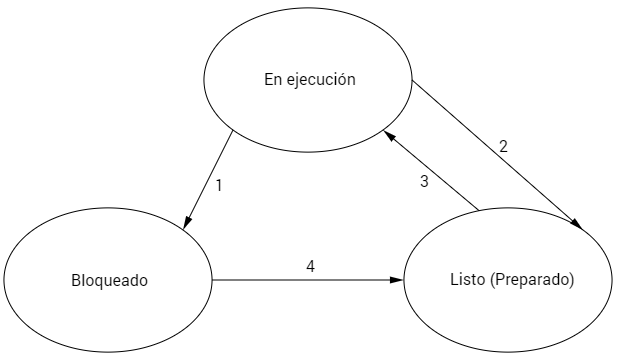
\includegraphics[width=\linewidth]{estados.png}

\end{minipage}

\textbf{Tipos de recursos:}

\begin{itemize}
\item \textit{Apropiativo:} el microprocesador puede ser compartido, ya sea por una \textit{interrupción} del \textit{timer} o porque llegó un proceso con mayor prioridad.

\item \textit{No apropiativo:} uso exclusivo de los recursos (proceso evoluciona a \textit{en espera} $\implies$ \textit{interrupción} $\implies$ se crea o termina un proceso).
\end{itemize}

\textbf{Métricas:}

\begin{enumerate}[a.]
\item \textit{Throughput:} procesos completados por unidad de tiempo.
\item \textit{Latency:} tiempo entre ocurrencia y respuesta de un evento.
\item \textit{Turnaround:} tiempo que una tarea necesita para completarse.
\item \textit{Waiting time:} tiempo de un proceso en cola estando \textit{listo}.
\item \textit{Fairness:} tiempo de espera/tiempo procesador.
\end{enumerate}

Los objetivos de los planificadores son minimizar el tiempo de respuesta, minimizar el \textit{throughput} (minimizar el \textit{overhead} y usar los recursos eficientemente), minimizar el tiempo de espera (equidad: que cada proceso espere la misma cantidad de tiempo). \\

\textbf{Políticas de clasificación:}

Lo habitual es usar políticas mixtas. Generalmente a corto plazo se usa \textit{round-robin}, mientras que a largo plazo varias colas FIFO.

\begin{itemize}
\item \textit{FIFO o FCFS:} los procesos se ejecutan según el orden de llegada, ejecutándose hasta que termine o ceda la CPU. Minimiza el \textit{overhead}, aunque es ineficiente cuando hay tareas que requieren poco tiempo de procesamiento detrás de una tarea que toma mucho tiempo.

\item \textit{Round-Robin:} los procesos toman turnos de un período limitado de tiempo para usar el microprocesador, ejecutando la primera tarea lista, estableciendo una \textit{interrupción} por \textit{timer} con una duración denominada \textit{quantum}. Al final del \textit{quantum}, si la tarea no se completó, la misma es apropiada y se le da la siguiente tarea lista al microprocesador. La tarea apropiada se pone en espera (estado \textit{listo}).

Se puede además establecer prioridades a las tareas, de manera de tener colas por prioridad y procesar primero la mayor prioridad. Esto presenta el potencial problema de inanición (proceso con prioridad baja que jamás se puede ejecutar), que se puede solucionar cambiando las prioridades en base al tiempo de procesamiento (bajar) o el tiempo de espera (subir).

\item \textit{Shortest Job First (SJF):} se ejecuta el trabajo con menor tiempo de procesamiento (estimado).

\item \textit{SRTF:} es una versión del SJF, pero apropiativo. Consiste en elegir siempre el proceso al que le reste menos tiempo de ejecución (CPU \textit{burst}). Minimiza el tiempo de respuesta promedio. Si todos los procesos tienen la misma duración SRTF es FIFO.
\end{itemize}

\dotfill \\

\textbf{Disco:}

Contiene uno o más platos que giran de 5400 a 10800 rpm. Posee un brazo mecánico (cabeza de lectura-escritura). Con un punto de giro colocado en una esquina. La información se escribe en el disco en una serie de círculos concéntricos. En cualquier posición del brazo, cada una de las cabezas puede leer una región llamada pista, y en conjunto todas las pistas dada una posición del brazo se denominan cilindro. Cada pista se divide en sectores (generalmente de 512 \textit{bytes}). Cuando se desplazan los brazos al encontrar la pista correcta, se espera a que el sector necesario se ubique debajo de ésta. Un \textit{cluster} es un conjunto de sectores. \\

\textbf{Memoria virtual:}

En los SO actuales, una parte del espacio de direcciones se mantiene en la memoria principal, y la otra parte en el disco. La memoria virtual sirve para ejecutar programas más extensos que la memoria física, llevando y trayendo pedazos entre la RAM y el HDD. \\

\textbf{Archivo:}

Colección de información relacionada y almacenada en un dispositivo de almacenamiento secundario de direcciones lógicas contiguas. Las estructura interna puede ser una secuencia de \textit{bytes} (Windows/Linux) o una secuencia de registros de longitud fija o variable. \\

\textbf{Tipos de archivos:}

\begin{itemize}
\item \textit{Regulares:} contienen información del usuario.
\item \textit{Directorios:} estructuras que permiten llevar el registro de los archivos. Pueden ser también archivos.
\item \textit{De dispositivo:} modelan dispositivos \textit{Input/Output} en serie. Ejemplo: impresoras, redes, etc.
\end{itemize}

\textbf{Forma de acceso a los archivos:}

\begin{itemize}
\item \textit{Secuencial:} un proceso puede leer todos los \textit{bytes} o registros en un orden, empezando del comienzo sin poder saltear pero sí rebobinar. Es el modo de acceso con cintas magnéticas.

\item \textit{Aleatorio:} leer \textit{bytes} o registros fuera de orden.
\end{itemize}

\textbf{Atributos de los archivos:}

\begin{itemize}
\item \textit{Nombre}.
\item \textit{Tipo}.
\item \textit{Localización (puntero)}.
\item \textit{Tamaño actual}.
\item \textit{Permisos (lectura, escritura,ejecución)}.
\item \textit{Fecha y hora}.
\end{itemize}

\textbf{Semánticas de consistencia:}

El SO administra la seguridad del sistema de manera que sea accesible sólo por usuarios autorizados. Específicamente las modificaciones de datos por un usuario se observan por otros usuarios. \\

\textbf{Funciones básicas de un sistema de archivos:}

Tener conocimiento de todos los archivos del sistema, controlar la compartición y forzar la protección de los archivos, gestionar el espacio de los sistemas de archivos y traducir direcciones lógicas de archivo a direcciones físicas. \\

\textbf{Implementación de un sistema de archivos:}

Aquí se define la forma en que se almacenan archivos y directorios, cómo se administra el espacio en disco y como hacer para que todo funcione con eficiencia y confiabilidad. Los SO poseen sus propios sistemas de archivos.

Los sistemas de archivos poseen dos problemas de diseño:

\begin{itemize}
\item Definir cómo el usuario ve el sistema de archivos.
\item Definir algoritmos y estructuras de datos que deben crearse para establecer una correspondencia entre el sistema de archivos (lógico) y los dispositivos físicos que los almacenan.
\end{itemize}

Las técnicas de implementación más usadas son: \\

\textbf{FAT:}

Este sistema de archivos usa una lista enlazada como estructura. La versión más reciente (FAT32) usa un arreglo de 32 bits en un área reservada del volumen. Cada archivo en el sistema se corresponde con una lista enlaza de entradas FAT. Cada entrada FAT contiene un puntero a la siguiente entrada FAT (o el valor \texttt{eof} para la última). La FAT posee una entrada para cada bloque en el volumen, y los bloques de archivo se corresponden con entradas de la FAT. \\

\textbf{Limitaciones de la FAT:}

\begin{enumerate}[a.]
\item Mala localidad (fragmentación).
\item Acceso aleatorio lento (ya que es una lista).
\item Metadatos limitados (no hay información sobre permisos, cualquier usuario puede manipular cualquier archivo).
\item Tamaño de archivo limitado (los tamaños de los archivos se codifican en 32 bits por lo que ningún archivo puede ser mayor a $2^{32}-1$ bytes $=4$ GB)
\end{enumerate}

\textbf{FFS:}

Usa índices basados en árboles multinivel, mejorando el acceso aleatorio. Además utiliza heurísticas de localidad para obtener buena localidad espacial. EXT2 y EXT3 están basados en FFS.

Para seguir el rastro de los bloques de datos que pertenecen a cada archivo, FFS usa un árbol asimétrico llamado \textit{multi-level index}. Cada archivo es un árbol con bloques de datos de tamaño fijo (por ejemplo, 4 KB) como hojas. Cada árbol (para cada archivo) comienza en un i-nodo, que posee los metadatos del archivo (dueño, permisos, fechas, si es una carpeta). El tamaño máximo de un archivo estará dado por la capacidad de direccionamiento del i-nodo. \\

\textbf{Estructura de un i-nodo:}

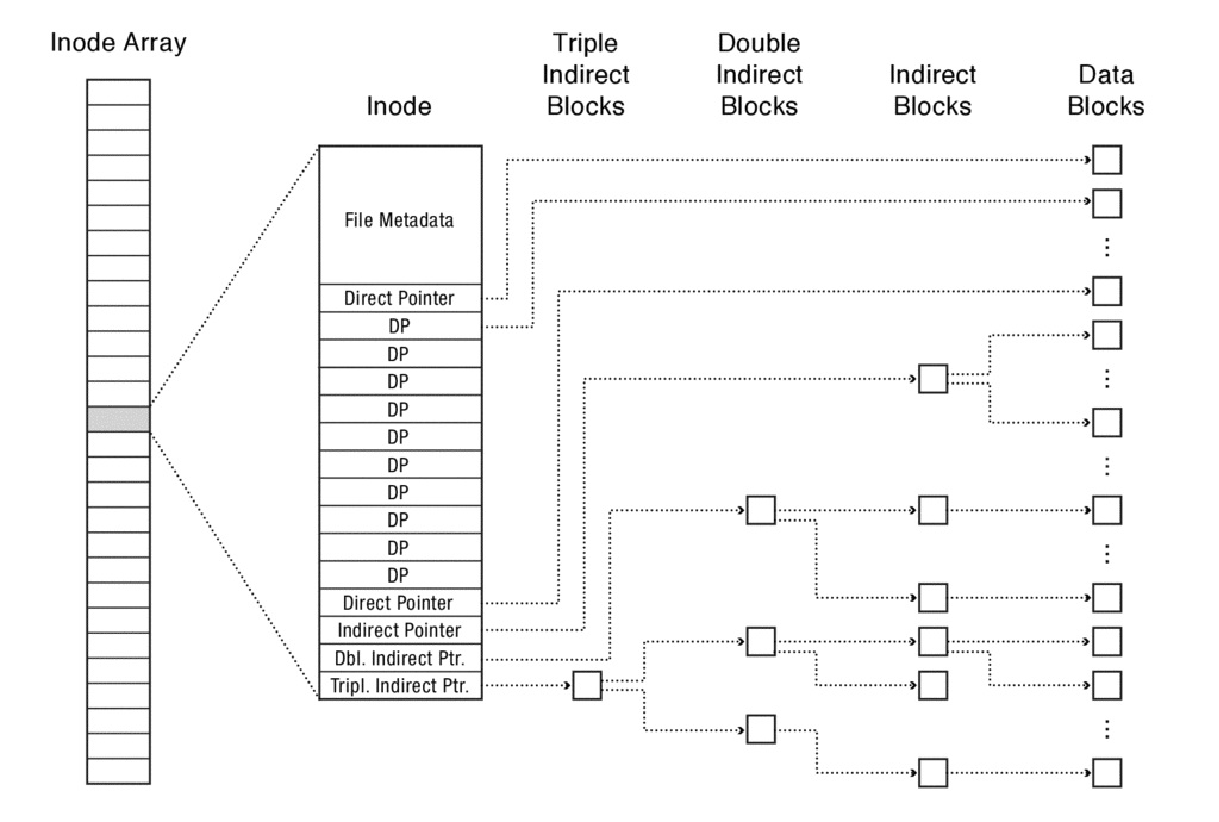
\includegraphics[width=\linewidth]{inodo}

Un archivo contiene un arreglo de punteros directos e indirectos:

\begin{itemize}
\item \textit{Punteros directos:} apuntan a los bloques de datos (hojas).

\item \textit{Punteros indirectos:}

	\begin{itemize}
	\item \textit{Simples:} apunta a un bloque de almacenamiento que posee un arreglo 		de punteros directos. Con bloques de 4 KB y punteros de 4 bytes, un bloque 				indirecto puede contener 1024 punteros directos (4 MB).
	
	\item \textit{Dobles:} apunta a un nodo interno del árbol llamado bloque doble 			indirecto (un arreglo de punteros indirectos que apuntan a un bloque indirecto). 		Con bloques de 4 KB, un puntero indirecto doble puede apuntar a $1024^{2}$ bloques 	de datos.
	
	\item \textit{Triples:} apuntan a bloques triples indirectos que contienen un 			arreglo de punteros indirectos dobles. Con bloques de 4 KB puede indexar $1024^{3}		$ bloques de datos que contienen $4[KB]\cdot 1024^{3}=2^{12}\cdot 2^{30}=2^{42}			=4[TB]$
	\end{itemize}

\end{itemize}

Todos los i-nodos del sistema se ubican en un arreglo de i-nodos que se almacena en una ubicación fija del disco. Cada archivo posee un número (\textit{i-number}) y ese número en FFS es un índice al arreglo de i-nodos. Para abrir un archivo se busca su i-nodo en un directorio y luego se busca la entrada apropiada en el arreglo de i-nodos para encontrar sus metadatos. \\

\textbf{Fragmentación:}

Memoria desperdiciada como consecuencia de las políticas de ajuste de bloques que tiene un sistema de archivos o la estructura del mismo.

\begin{quote}

\textbf{Tipos de fragmentación:}
\begin{itemize}
\item \textit{Interna:} se da cuando el tamaño de un archivo (o la diferencia entre el tamaño de una cantidad entera de \textit{clusters}) es menor que al tamaño del \textit{cluster} (el \textit{cluster} entero se reserva para ese archivo por más que no esté completamente ocupado).

\item \textit{Externa:} ocurre luego de la sucesiva creación y eliminación de archivos de distintos tamaños, aislando bloques libres, y cuando la política de ajuste del disco no elige a estos bloques para nuevos archivos.
\end{itemize}

\end{quote}

\textbf{Planificación de discos:}

Los algoritmos de planificación intentan minimizar el tiempo de búsqueda. La efectividad se mide sumando la diferencia de pistas entre cada solicitud y dividiendo por la cantidad de solicitudes. \\

\begin{quote}
\begin{itemize}
\item \textit{FCFS (FIFO):} las solicitudes se procesan en un orden secuencial. Es justa para todos los procesos. Si hay muchos procesos es similar a una técnica aleatoria.

\item \textit{SSTF:} primero se procesan las peticiones que minimizan el movimiento de cabezas desde la posición actual. Puede causar inanición.

\item \textit{SCAN:} el movimiento del brazo empieza en un extremo y continúa hasta el otro. Allí se cambia el sentido y se vuelve al otro extremo atendiendo tareas a la vuelta.

\item \textit{C-SCAN:} las cabezas se mueven de un extremo al otro del disco y luego vuelven al principio. No se atienden peticiones mientras las cabezas vuelven a la posición inicial (ir del último al primero es más rápido que ir parando). 
\end{itemize}
\end{quote}

\section{Preguntas}

\begin{enumerate}[1.]
\item ¿Es posible que un proceso a nivel de \textit{usuario} logre privilegios del \textit{kernel}? Justifique.

\begin{quote}
No, ya que al estar a nivel de \textit{usuario} el microprocesador no permite que se ejecuten instrucciones del \textit{kernel}. Lo que se puede hacer es avisar al sistema operativo de alguna forma que se quiere ejecutar una instrucción privilegiada, ya que este si posee privilegios de \textit{kernel}. Esto se puede hacer mediante \textit{llamadas al sistema (trap)}.
\end{quote}

\item ¿Qué diferencia existe entre una \textit{llamada al sistema (trap)} y una invocación a un procedimiento convencional? Justifique.

\begin{quote}
Una invocación a un procedimiento (función) se realiza en \textit{modo usuario} desde el inicio hasta el fin, mientras que en una \textit{llamada al sistema (trap)} esta instrucción cambia el modo del microprocesador a \textit{modo kernel} y ejecuta una serie de instrucciones siguiendo un \textit{handler} que le pone límites.
\end{quote}

\item Asuma que un sistema tiene que planificar la asignación de la CPU en forma \textit{justa} a un conjunto de tareas, algunas de las cuales tienen un alto requerimiento de CPU y otras, una alta demanda de E/S ¿a qué tipo de tareas daría más prioridad? El mecanismo SRTF consiste en asignar la CPU al trabajo que tenga un duración menor. Dado que es imposible conocer la duración exacta de una tarea, ¿de qué manera se resuelve esto?

\begin{quote}
La asignación de la CPU es \textit{justa} cuando los procesos son atendidos en orden de llegada. \\

La prioridad de las tareas dependerá del planificador de procesos, en este caso FCFS (FIFO). Mientras un programa está siendo ejecutado por el microprocesador otro se carga en memoria a través de los dispositivos \textit{input/output} mediante el DMA (\textit{acceso directo a memoria}). \\

El DMA permite leer y escribir en la memoria independientemente del microprocesador. \\

El mecanismo SRTF determina cuáles son los tiempos de las tareas mediante estimaciones estadísticas.
\end{quote}

\item ¿Qué tipo de evento(s) provoca la evolución de un proceso del estado \textit{en ejecución} a \textit{listo}? ¿Es posible que un proceso evolucione desde un estado bloqueado a un estado en ejecución? Justifique.

\begin{quote}
Esta evolución se da cuando ocurre una \textit{interrupción} por el \textit{timer}. Esta es una forma de que el sistema operativo tome el control del proceso para hacer algo con éste o cambiar a otra tarea. El hardware interrumpe el microprocesador cada cierto tiempo o cantidad de instrucciones. Si hay un mecanismo de planificación activo que use \textit{quantos} de tiempo (por ejemplo, \textit{Round Robin}), el control pasará al siguiente proceso de igual prioridad cambiando el estado del proceso actual de \textit{en ejecución} a \textit{listo}. \\

No, no es posible. Para llegar del estado \textit{bloqueado} al estado \textit{en ejecución}, los procesos primero deben pasar al estado \textit{listo}. Los procesos bloqueados están a la espera de un \textit{evento} que de llegar cambia el estado de \textit{bloqueado} a \textit{listo}, para ser ejecutado según el planificador.
\end{quote}

\item Cuando se invoca una \textit{llamada al sistema} (system call), el control evoluciona, en algún momento, de la \textit{capa usuario} a la \textit{capa kernel}. Detalle en forma de \textsc{pseudocódigo} la manera en que se concretan tales cambios de privilegios considerando las estructuras de datos involucradas.

\begin{quote}

Se puede proveer una librería que encapsule las \textit{llamadas al sistema} mediante un \textit{stub} ubicado en la región de memoria del \textit{kernel}, por lo que este \textit{stub} hace la llamada al sistema con privilegios. Por ejemplo, para abrir un archivo:

\begin{enumerate}[1.]
\item \texttt{El programa de usuario llama al \textit{stub} como a cualquier función (sin saber que esa función realiza instrucciones en \textit{modo kernel}).}

\item \texttt{El \textit{stub} llena el código necesario para la \textit{llamada al sistema} y ejecuta la \\ instrucción \textit{trap}.}

\item \texttt{El harware transfiere el control al \textit{kernel} a través del \textit{handler} para llamadas externas. El \textit{handler} actúa como un \textit{stub} pero del lado del \textit{kernel}, copiando y verificando los argumentos y luego llamando a la implementación de la \textit{llamada al sistema} en el \textit{kernel}.}

\item \texttt{Luego de que se completa la \textit{llamada al sistema} se vuelve con el resultado al \textit{handler}.}

\item \texttt{El \textit{handler} vuelve al \textit{modo usuario} pero a la siguiente instrucción del \textit{stub}.}

\item \texttt{El \textit{stub} devuelve el resultado a la función original.}
\end{enumerate}

\end{quote}

\item ¿Por qué entiende las variables locales se almacenan en la pila en lugar de en un segmento de memoria convencional?

\begin{quote}
Las variables locales al poder referenciarse sólo en la función en las que se las han declarado, deben existir sólo durante la ejecución de la función que la declara. Por esto, la mejor estructura para modelar este comportamiento es un \textit{pila} ya que primero se insertan las variables de las funciones externas y cuando se procesa la última función interna, en el tope de la pila quedan las variables de esta función que posteriormente serán eliminadas
\end{quote}

\item Detalle las \textsc{estructuras de datos} que provee el \textit{kernel} en un sistema de i-nodos para gestionar los archivos y el rol de cada una. Explique a través de un \textsc{pseudocódigo} el uso de las mismas cuando se realice una operación de escritura de un archivo. Considere que el i-nodo tiene dos enlaces directos y uno indirecto simple con 2 enlaces.

\begin{quote}
Los i-nodos constan de una estructura de árbol multinivel. 

\begin{itemize}
\item El \textit{super bloque} contiene información referente al estado del disco y a las particiones de los datos.

\item El \textit{bitmap i-nodo} se utiliza para indicar el estado de los i-nodos y ver si están ocupados o libres.

\item El \textit{bitmap bloques} se utiliza para indicar el estado de los bloques y ver si están ocupados o libres.

\item Todos los i-nodos de los archivos del sistema se ubican en un \textit{arreglo} de i-nodos que se almacena en una ubicación fija del disco. Un i-nodo contiene enlaces directos, enlaces indirectos simples, enlaces indirectos dobles y enlaces indirectos tripes. Los enlaces directos apuntan a bloques de datos. Los enlaces indirectos simples apuntan a bloques de puntero que apuntan a bloques de datos. Los enlaces indirectos dobles apuntan a bloques de enlaces indirectos simples. Los enlaces indirectos triples apuntan a bloques de enlaces indirectos dobles.

\item Todos los bloques de datos de los archivos del sistema se ubican en un \textit{arreglo} de bloques que se almacena en una ubicación fija del disco.
\end{itemize}

\begin{enumerate}[1.]
\item \texttt{Primero se intentan ocupar los bloques de datos pertenecientes a los bloques directos.}

\item \texttt{Si los bloques de los enlaces directos no son suficientes se pasan a utilizar los bloques de datos de los enlaces indirectos simples hasta almacenar el \\ archivo completo.}
\end{enumerate}
\end{quote}

\item ¿Qué objetivos intentan satisfacer las arquitecturas de sistemas operativos monolítica y \textit{microkernel}?

\begin{quote}
\textit{Microkernel}: las partes menos críticas del sistema operativo (por ejemplo, el sistema de archivos o las ventanas) se aíslan del resto del \textit{kernel}, resultando en un \textit{kernel} pequeño. Esto permite tener un \textit{kernel} más dinámico, en el cual se pueden agregar características sin tener que recompilar todo el \textit{kernel}. Al tener esta división entre \textit{kernel} y librerías se obtiene un rendimiento menor que en los monolíticos, pero la división misma otorga confiabilidad ya que una falla de una de las librerías no afecta a todo el sistema. \\

\textit{Monilítico:} en éste, todas las partes del sistema operativo se almacenan en el espacio del \textit{kernel}, resultando más rápidos que los anteriores pero más vulnerables a fallas del sistema.
\end{quote}

\end{enumerate}






\end{document}